\csname documentclass\endcsname[../main.tex]{subfiles}
\begin{document}
\appendix

\chapter{Dataset Details}\label{appendix:datasets}

\chapter{Greedy Optimal and True Optimal}\label{appendix:optimal-policies}

We train an IntCEM according to Zarlenga et al.~\cite{intcem}, 
and evaluate the intervention performance when using
Greedy Optimal and True Optimal. 
Figure~\ref{fig:greedy-vs-optimal} shows the test performance of 
Greedy Optimal and True Optimal on an IntCEM for the 
MNIST-ADD task. We see that True Optimal outperforms 
Greedy Optimal for all intervention groups, except
when only 1 group is intervened and when 8 groups are intervened
since the non-greedy and greedy optimal policies 
makes the same interventions for these two scenarios. 

\begin{figure}[!h]
    \centering
    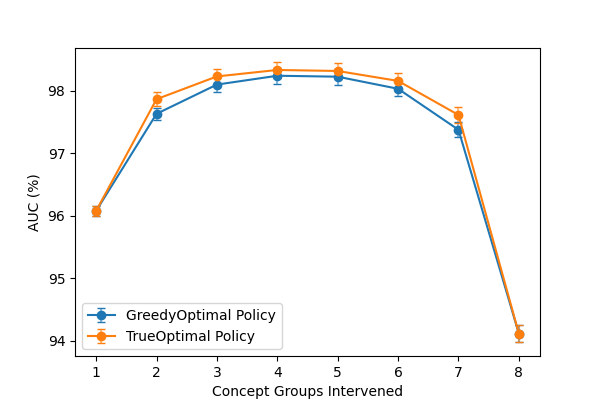
\includegraphics[width=0.9\textwidth]{figs/evaluation/greedy_vs_true_optimal.png}
    \caption{
        Test Intervention AUC (\%) of GreedyOptimal and TrueOptimal
        on an IntCEM trained on MNIST-ADD. GreedyOptimal and TrueOptimal are the greedy and non-greedy optimal intervention
        policies respectively.
    }
    \label{fig:greedy-vs-optimal}
\end{figure}

The reason the performance when using
fewer interventions (e.g. when 4 groups are intervened) is higher than
when more groups are intervened (e.g. when all groups are intervened)
is because the intervention policies have access to the true 
label, and can cherry-pick interventions that result in 
the prediction to align more with the true label. This is
normal for a policy that has access to the 
true labels, and as we can see in 
Section~\ref{eval:rlcem-performance}, this behaviour is not observed 
in learnt policies such as IntCEM or RLCEM.
\chapter{Surrogate Model Details}

\section{Transformations}\label{appendix:transformations}

\section{Hyperparameters}\label{appendix:surrogate-hyperparameters}

\chapter{Hardware Specifications}

% \chapter{Training Graphs}\label{appendix:training-graphs}

\chapter{L2 Penalty}\label{appendix:l2-penalty}
\end{document}